\documentclass[10pt,a4paper]{article}
\usepackage[margin=2.2cm]{geometry}
\usepackage{amsmath,amssymb,graphicx,booktabs,caption,float,xcolor,enumitem}
\usepackage[colorlinks=true,linkcolor=blue!50!black,urlcolor=blue!50!black]{hyperref}
\captionsetup{font=small,labelfont=bf}
\setlist{itemsep=1pt,topsep=3pt}
\graphicspath{{figures/}}

\title{\textbf{What sets where the reading reversal happens?}\\[2pt]
\textbf{The agents' counter-evidence}}
\author{Claude (theory work, \nolinkurl{analysis/theory_claude/phenomenological_fact_flow/})}
\date{28 October 2026}

\begin{document}
\maketitle

\begin{abstract}
\noindent
The four simulator setups reverse at different memories. Object Placements symmetric reverses at short memory, then
task003 symmetric, then the two no-proof setups at long memory. Completed proofs are too rare to explain this (report of
28 October). The fact-flow model suggests a different cause: how strongly the agents' own evidence argues against the
wrong answer. We measured this strength in each setup from stored simulator memories, with the prediction fixed before
measuring. The four strengths come out in exactly the reverse order of the four crossovers. Putting the measured
strengths into the model, with nothing fitted to the reversal, reproduces the symmetric/no-proof contrast in both tasks
and the task difference among symmetric setups, but swaps the two no-proof setups.
\end{abstract}

\section{The idea}
In the fact-flow model the reversal is a contest between \emph{dose} and \emph{sensitivity}:
\begin{equation}
D\approx\beta_C\,\sigma'(x_s)\Big[\underbrace{\Delta M_C}_{\text{dose}}-\underbrace{(1-2\Phi_s)\,\beta_A\,M_C\,\Delta M_A}_{\text{sensitivity loss}}\Big],\qquad x=h_0+\beta_C M_C-\beta_A M_A.\label{eq:D}
\end{equation}
Reading more raises the controller's dose $M_C$. It also adds the agents' own evidence $M_A$, which pulls the population
away from the wrong answer and makes it less sensitive. The second term is proportional to $\beta_A$, the
\emph{counter-evidence strength}: how much each of the agents' own facts lowers the log-odds of the wrong answer. A larger
$\beta_A$ lets the protective side win at shorter memory, so the crossover moves to shorter memory.

\section{Measurement and predictions (fixed before measuring)}
For each setup we took every stored agent memory $M$ at $t=30$: false arm, $q=6$, $\rho\in\{0.25,0.5,0.75\}$, 72{,}000
memories per setup. We computed the exact belief $P(A2\mid M)$ and fitted, by least squares,
\begin{equation}
\operatorname{logit}P(A2\mid M)=h_0+\beta_C\,c(M)-\beta_A\,a(M),\label{eq:fit}
\end{equation}
where $a$ and $c$ are the numbers of agent facts and controller facts held. $P$ is clipped to $[10^{-3},1-10^{-3}]$,
because a proof gives $P(A2)=0$. No vote, effect size or reversal enters this measurement. Predictions:
\begin{itemize}
\item[B1] $\beta_A$ is larger in the symmetric setup than in the no-proof setup of the same task.
\item[B2] The four $\beta_A$ are ordered as the reverse of the four simulator crossovers.
\item[B3] The model, given the measured $(h_0,\beta_A,\beta_C)$ and nothing else changed, orders its crossovers in the
  same way.
\end{itemize}

\section{Results}
\begin{table}[h]
\centering\small
\begin{tabular}{@{}lcccccc@{}}
\toprule
setup & $\beta_A$ & $\beta_C$ & $h_0$ & simulator crossover $3\to6$ & model crossover\\
\midrule
Object Placements, symmetric & \textbf{1.14} & 0.86 & $-0.72$ & 0.25--0.375 & below 0.05\\
task003, symmetric & \textbf{0.67} & 0.63 & $-0.13$ & 0.5--0.625 & 0.2--0.25\\
Object Placements, no-proof & \textbf{$-0.07$} & 0.14 & $-0.71$ & 0.625--0.875 & none (above 0.99)\\
task003, no-proof & \textbf{$-0.17$} & 0.38 & $-0.46$ & 0.75--1 & 0.85--0.9\\
\bottomrule
\end{tabular}
\caption{Measured strengths and crossovers. Rows are ordered by the simulator's crossover.}
\label{tab:res}
\end{table}

\begin{figure}[h]
\centering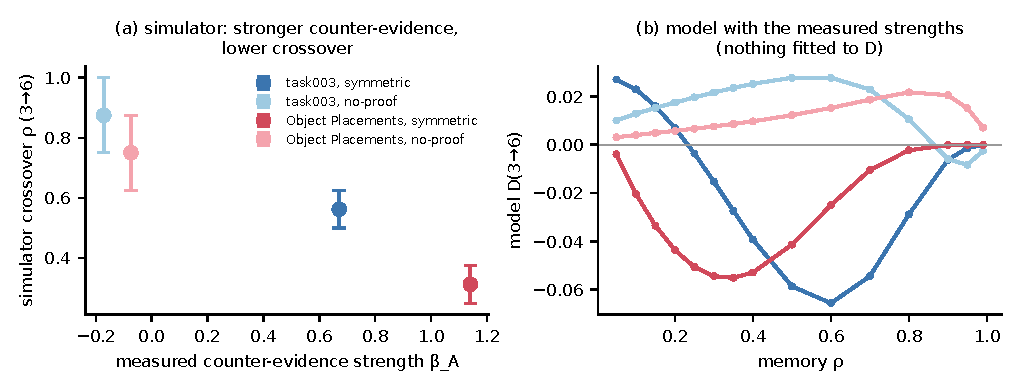
\includegraphics[width=\linewidth]{fig1_counterevidence.pdf}
\caption{\textbf{(a)} In the simulator, setups whose agents hold stronger counter-evidence reverse at shorter memory
(bars: the $\rho$ interval in which the sign of $D(3\to6)$ changes). \textbf{(b)} The fact-flow model with each setup's
measured strengths: symmetric setups reverse at short memory and no-proof setups at long memory or not at all.}
\label{fig:ce}
\end{figure}

\begin{itemize}
\item \textbf{B1 met, by a wide margin.} In the symmetric setups each agent fact lowers the log-odds of the wrong answer
  (0.67 and 1.14). In the no-proof setups it slightly \emph{raises} them ($-0.07$ and $-0.17$). This is because the
  agents' facts together point to an even split between the right and the wrong answer: accumulating them makes the
  wrong answer more likely than the prior 1/3.
\item \textbf{B2 met exactly.} The order of $\beta_A$ is the reverse of the order of the crossovers
  (Fig.~\ref{fig:ce}a). A secondary measure, the mean change in log-odds when one random agent fact is added, ranks the
  two symmetric setups the other way (0.18 against 0.24). The prediction was stated for the primary measure.
\item \textbf{B3 partly met} (Fig.~\ref{fig:ce}b):
  \begin{itemize}
  \item symmetric below no-proof within each task: met;
  \item Object Placements below task003 among the symmetric setups: met;
  \item the two no-proof setups are swapped. Their $\beta_A$ differ little, and their model curves are nearly flat, so
    $\beta_C$ and $h_0$ decide between them.
  \end{itemize}
  The model's crossovers sit at shorter memory than the simulator's; positions were not a target.
\end{itemize}

\section{What this means}
One measured number, the agents' counter-evidence strength, orders where the four setups reverse. It explains the main
contrast with a mechanism rather than a proof count:
\begin{itemize}
\item when the swarm's own evidence argues against the controller (symmetric setups), reading helps the swarm already at
  short memory;
\item when it does not (no-proof setups, whose evidence points to an even split), reading protects only at long memory,
  through the slower loss of sensitivity.
\end{itemize}
Proofs are not needed. Their role in the symmetric setups is to make the agents' facts argue against the wrong answer,
which they do long before any agent holds a complete proof.

\paragraph{Caveats.}
\begin{itemize}
\item The fit~\eqref{eq:fit} is a linear summary of a non-linear, context-dependent belief, so $\beta_A$ is an average
  over the memories that actually occur.
\item The secondary measure disagrees on the order within the symmetric pair.
\item The model's no-proof order is wrong.
\item The measurement uses memories from the same runs as the crossovers, but no vote or effect size, so it is
  independent of the quantity being explained, not of the runs.
\end{itemize}

\section{Next steps}
\begin{enumerate}
\item \textbf{A finite fact-flow model} (planned): whole numbers of holders and copies, so facts can die out. It tests the
  diversity collapse, the size of $G$, the residual after removal and the slow fading of persistence.
\item \textbf{A formula for the crossover} from Eq.~\eqref{eq:D}, now with a concrete target: the crossover should fall as
  $\beta_A$ grows, and as $q$ grows.
\end{enumerate}

\end{document}
